% Chapter 3

\chapter{Simulation 2D} % 3rd chapter title

\label{Chapter3} % For referencing the chapter elsewhere, use \ref{Chapter3} 

%----------------------------------------------------------------------------------------

Ayant simulé le schéma de « splitting » en 1D avant le stage, on s'intéresse dans cette partie à sa simulation en 2D. Il s'agit donc de résoudre le problème direct du transfert radiatif avant de passer au problème inverse dans le chapitre suivant. On rappelle brièvement l'équation du transfert radiatif (ETR), le modèle P1 couplé avec la matière, le schéma de « splitting », avant de présenter l'implémentation en C++.

\section{Le transfert radiatif}

On considère un rayonnement transporté par des particules de masse nulle appelés photons. Lorsqu'ils se trouvent en présence de la matière, les photons interagissent avec les atomes. Trois phénomènes sont prépondérants (figure \ref{fig:TransferRadiatif}) :

\begin{figure}[!h]
\centering
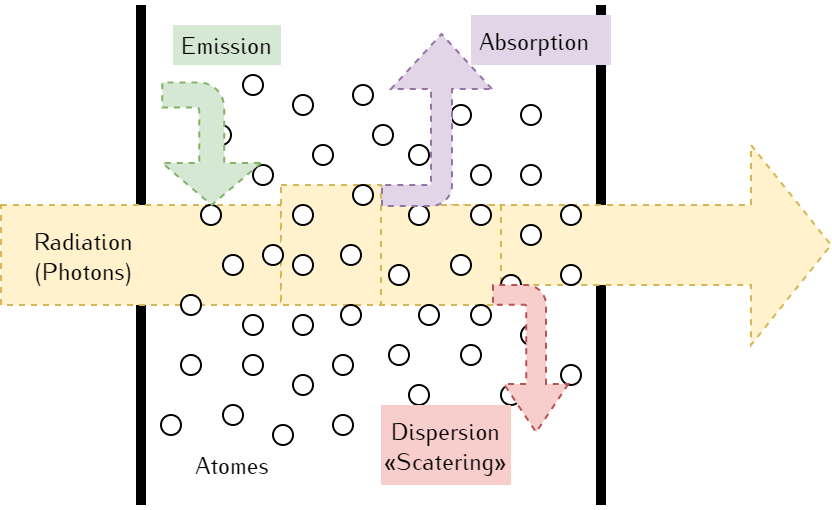
\includegraphics[width=.5\linewidth]{TransferRadiatif} 
\decoRule
\caption[TransferRadiatif]{Illustration des interactions entre radiation et matière.}
\label{fig:TransferRadiatif}
\end{figure}

\begin{itemize}
 \item L'\textbf{émission} : des photons sont émis en réponse aux électrons excités descendants à des niveaux d'énergie plus bas. Ce phénomène est caractérisé par l'opacité d'émission $\sigma_e$. Il s'agit de l'inverse du libre parcours moyen d'émission \footnote{Le libre pacours moyen d'émission represente la distance moyenne entre deux émissions consecutives de photons. Les libres parcours moyen d'absorption et de dispersion sont définis de maniere similaire.}. Plus la température matière est élevée, plus ce phénomène est important.
 \item L'\textbf{absorption} : à l'inverse, certains photons sont absorbés, les électrons deviennent plus excités (ou se libèrent complètement de leurs atomes), et la matière se réchauffe. Ce phénomène se caractérise par l'opacité d'absorption $\sigma_a$. Lorsqu'on est à l'équilibre thermique, $\sigma_a = \sigma_e$.
 \item La \textbf{dispersion} (ou « \textbf{scattering} » ou parfois \textbf{diffusion}) : certains photons sont déviés de leur trajectoire originale par la matière. Ce phénomène se caractérise non seulement par son opacité de « scattering » $\sigma_c$ \footnote{ $\sigma_a$ et $\sigma_c$ sont definis de manière similaire à $\sigma_e$}, mais aussi par une fonction de distribution angulaire décrivant la manière dont les photons sont déviés \parencite[13]{Reference3}.
\end{itemize}

L'équation du transfert radiatif (ETR) (équation \ref{eqn:ETR}) représente un bilan d'énergie lié au rayonnement au niveau microscopique. Nous nous placerons dans le cas particulier d'équilibre thermodynamique local (ETL)\footnote{État dans lequel on peut définir une température pour chaque point du domaine, et l'émission est décrite par la fonction de Planck \parencite{Reference3}.}. L'équilibre radiatif \footnote{Il se produit si la matière est à l'équilibre avec le rayonnement. Si on est dans l'ETL, les photons sont émis suivant la fonction de Planck à la température de la manière.} quant à lui sera considéré plus tard comme condition initiale pour les simulations.
\begingroup
\footnotesize
\begin{gather}
    \begin{aligned}
    \frac{1}{c} \frac{\partial}{\partial t}I(t,\bvec{x},\bm{\Omega},\nu)+\bm{\Omega}\cdot\nabla_{\bvec{x}} I(t,\bvec{x},\bm{\Omega},\nu)
    &= \sigma_a(\rho,\bm{\Omega},\nu)\left(B(\nu,T)-I(t,\bvec{x},\bm{\Omega},\nu)\right) \\
    &+ \frac{1}{4\pi} \int_{0}^{\infty} \int_{S^2}\sigma_c(\rho,\bm{\Omega},\nu)p(\bm{\Omega}^\prime\rightarrow\bm{\Omega})\left(I(t,\bvec{x},\bm{\Omega}^\prime,\nu)-I(t,\bvec{x},\bm{\Omega},\nu)\right) \, d\bm{\Omega}^\prime \, d\nu
    \end{aligned}
\label{eqn:ETR}
\end{gather}
\endgroup
Où $I$ est l'intensité spécifique de radiation et $p$ est la fonction de distribution angulaire de « scattering » (telle que $\oint p(\bm{\Omega}^\prime\rightarrow\bm{\Omega})\, d\bm{\Omega}^\prime=1$). Les autres termes sont définis dans la liste des symboles de la page \ref{sec:symbols}.

Plusieurs modèles ont été créés pour modéliser l'ETR avec différents niveaux de précision. Le modèle P1 est un modèle macroscopique \footnote{Il ne prend en compte que les variables d'espace et de temps et est obtenu par intégration de termes microscopique tels que $I$ par rapport à la fréquence et la direction.} aux moments (d'ordre 2), linéaire et hyperbolique. Vu que l'énergie du rayonnement n'est pas conservée durant son interaction avec la matière, il faut coupler le modèle P1 avec une équation régissant l'énergie de la matière. On utilisera une équation d'énergie matière simplifiée qui ne tient compte que des termes d'échange avec le rayonnement. Le modèle P1 couplé avec la matière est présenté ci-bas \parencite{Reference2} :
\begingroup
\large
\begin{equation}
    \begin{cases}
     \partial_tE + c \ \operatorname {div} \bvec F = c\sigma_a\left(aT^4-E\right)\\
     \partial_t\bm{F} + c \ \nabla E = -c\sigma_c \bvec{F} \\
     \rho C_v \partial_t T = c \sigma_a \left(E-aT^4\right)
    \end{cases}
\label{eqn:P1}
\end{equation}
\endgroup
Dans l'équation \ref{eqn:P1}, $\sigma_a$ et $\sigma_c$ sont écrits sans indiquer leurs arguments \footnote{Juste $\rho$ et $T$ si on se place dans l'ETL.} afin de faciliter la lisibilité. $E$, $F$, et $T$ représentent l'énergie des photons, le flux de photons, et la température matière. Partant de l'équation \ref{eqn:ETR}, $E$ et $T$ sont définis de la manière suivante :
\begin{align*}
E(t,\bvec{x}) &= \frac{4\pi}{c} \int_{0}^{\infty} \int_{S^2} I(t,\bvec{x},\bm{\Omega},\nu) \, d\bm{\Omega} \, d\nu \\
\bvec{F}(t,\bvec{x}) &= \frac{4\pi}{c} \int_{0}^{\infty} \int_{S^2} \bm{\Omega}I(t,\bvec{x},\bm{\Omega},\nu) \, d\bm{\Omega} \, d\nu 
\label{eqn:EFT}
\end{align*}

Comme on peut le voir à travers la définition de $E$ et $F$, notre modèle est dit "gris" car nous l'intégrons sur tout le spectre de fréquence. En effet, nous nous intéressons au rayonnement à travers son bilan d'énergie transporté par le flux radiatif. Sur ce point, la version du modèle P1 que nous avons utilisé est mois précise qu'un modèle microscopique basé soit sur une méthode de Monte-Carlo ou une méthode des ordonnées discrètes. Néanmoins notre modèle présente l'avantage d'être très peu couteux et relativement facile à implémenter \parencite{Reference3}. 

%----------------------------------------------------------------------------------------

\section{Schéma de splitting}

Le modèle P1 tend vers une équation de diffusion lorsque les opacités d'absorption ($\sigma_a$) et de dispersion ($\sigma_c$) sont élevées (de façon à ce que $c/\sigma_a \approx 1$). Ce cas limite est appelé \textbf{approximation de diffusion} et est indiqué à l'équation \ref{eqn:Diff}.
\begin{equation}
\partial_t \left( aT^4 + \rho C_v T \right) - \operatorname{div} \left(\frac{acT^3}{\sigma_a} \nabla T \right) = O\left( \frac{1}{c} \right)
\label{eqn:Diff}
\end{equation}
Les schémas classiques tels que le schéma de Rusanov ne sont pas assez précis pour capturer cette propriété. Le schéma en deux étapes (ou de « splitting ») proposé par M. \textsc{Franck} permet de pallier ce problème. Ses deux étapes sont résumées ci-bas \parencite{Reference4}.


\subsection{Etape 1}
La première étape (dite étape de couplage ou d'équilibre, ou de relaxation de la température) permet de régler la température sur chaque maille (indépendamment des autres mailles). On ne considère que les équations où la température est impliquée (EDP 1 et 3 du système d'équation \ref{eqn:P1}), en fixant la valeur du flux sur chaque maille. Il s'agit d'une méthode de point fixe qui est toujours définie \parencite{Reference2}.

Le domaine rectangulaire est supposé discrétisé en $N \times M$ mailles uniformes ; on se trouve sur la maille $j$ (voir figure \ref{fig:Discretisation2D} pour les détails de la discrétisation) à l'étape d'itération $n$. On pose donc $\Theta = aT^4$ et on obtient le système :
\begingroup
\normalsize
\begin{equation*}
    \begin{dcases}
     \dfrac{E_j^{q+1} - E_j^{n}}{\Delta t} = c \sigma_a ( \Theta_j^{q+1} - E_j^{q+1}) \\
     \rho_j C_v \mu_q \dfrac{\Theta_j^{q+1} - \Theta_j^{n}}{\Delta t} = c \sigma_a (E_j^{q+1} - \Theta_j^{q+1}) 
    \end{dcases}
% \label{eqn:Step1}
\end{equation*}
\endgroup
Où $\mu_q = \dfrac{1}{T^{3,n} + T^{n}T^{2,q} + T^{q}T^{2,n} + T^{3,q}}$.

L'étape revient à résoudre un système de Cramer. On obtient donc :
\begin{equation} 
    \begin{dcases}
     E_j^{q+1} = \dfrac{\alpha E_j^n + \beta \gamma \Theta_j^n}{1 - \beta \delta} \\
     \Theta_j^{q+1} = \dfrac{\gamma \Theta_j^n + \alpha \delta E_j^n}{1 - \beta \delta} 
    \end{dcases}
\label{eqn:Step1}
\end{equation}
Avec $\quad  \alpha = \dfrac{1}{\Delta t \left( \frac{1}{\Delta t} + c \sigma_a \right)} ,\quad 
\beta = \dfrac{c \sigma_a}{\frac{1}{\Delta t} + c \sigma_a} ,\quad 
\gamma = \dfrac{\rho_j C_v \mu_q}{\Delta t \left( \frac{\rho_j C_v \mu_q}{\Delta t} + c \sigma_a \right)} \quad \text{et} \quad  
\delta = \dfrac{c \sigma_a}{\frac{\rho_j C_v \mu_q}{\Delta t} + c \sigma_a}.$

On itère ainsi sur $q$ jusqu'à ce que $E$ et $\Theta$ convergent respectivement vers $E^*$ et $\Theta^*$. $F$ reste inchangé durant cette étape.

\subsection{Etape 2}
Il s'agit ici de résoudre les deux premières EDP du système d'équation \ref{eqn:P1}. Avant d'attaquer le schéma de « splitting », on note que les équations à résoudre sont hyperboliques et que la méthode des volumes finis est donc la mieux adaptée. On se place sur une maille $j$ caractérisée par son volume $\Omega_j$ \footnote{On utilisera généralement le terme "maille" vu qu'en 2D, le "volume" $\Omega_j$ est en réalité une surface.}.
\begin{equation*} 
    \begin{dcases}
    \partial_t \int_{\Omega_j} E + c \int_{\Omega_j} \operatorname{div} \bvec F  = 0\\
    \partial_t \int_{\Omega_j} \bvec{F} + c \int_{\Omega_j} \nabla E = -c \sigma_c \int_{\Omega_j} \bvec F 
    \end{dcases}   
% \label{eqn:VolFin}
\end{equation*}
On définit une normale $\bvec n_j$ à la surface $\Omega_j$ \footnote{Il s'agit en réalité d'une série de quatre normales définies par rapport aux mailles voisines de $j$ (voir figure \ref{fig:Interaction2D}).} et on applique le théorème de la divergence. On moyenne les intégrales sur chaque maille pour obtenir :
\begin{equation} 
    \begin{dcases}
    \partial_t E_j + \frac{c}{\left|\Omega_j\right|} \int_{\partial\Omega_j} \left( \bvec F, \bvec n_j  \right) = 0\\
    \partial_t \bvec{F}_j + \frac{c}{\left|\Omega_j\right|} \int_{\partial\Omega_j} \left( E, \bvec n_j  \right)= \frac{c \sigma_c}{\left|\Omega_j\right|} \int_{\Omega_j} \bvec F
    \end{dcases}   
\label{eqn:VolFin}
\end{equation}
Avec $$ E_j(t) = \frac{1}{\left|\Omega_j\right|} \int_{\Omega_j} E(t,\bvec x) \quad \text{et} \quad \bvec F_j(t) = \frac{1}{\left|\Omega_j\right|} \int_{\Omega_j} \bvec F(t,\bvec x) $$

Nous devons maintenant retourner sur le maillage en définissant les différents flux numériques impliqués. Durant cette étape, il faut considérer l'ajout de mailles fantômes (figure \ref{fig:Discretisation2D}), ce qui porte le nombre total de mailles à $(N+2) \times (M+2)$.

\begin{figure}[H]
\begin{subfigure}{.6\textwidth}
  \centering
  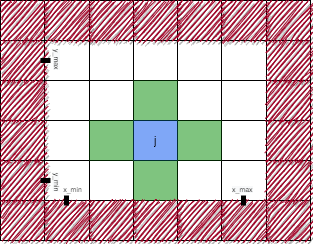
\includegraphics[width=.8\linewidth]{Dicretisation2D}  
  \caption{Maillage 2D}
  \label{fig:Discretisation2D}
\end{subfigure}
\begin{subfigure}{.4\textwidth}
  \centering
  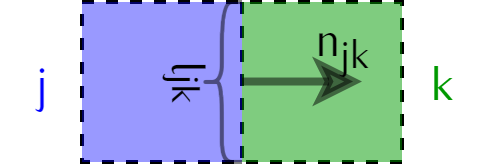
\includegraphics[width=.8\linewidth]{Interaction2D}  
  \caption{Interaction entre deux mailles j et k}
  \label{fig:Interaction2D}
\end{subfigure}

\centering
\decoRule
\caption{Discrétisation du maillage 2D. Sur la figure (A), on peut observer les mailles dites "fantômes" hachurées en rouge. Les quatre mailles voisines d'une maille $j$ sont indiquées en vert. Les nombres de mailles suivant la verticale $N$ et suivant l'horizontale $M$ sont choisis telle que le maillage soit uniforme i.e $\Delta x = \frac{x_{max}-x_{min}}{N} = \frac{y_{max}-y_{min}}{M} = \Delta y$. Sur la figure (B), on observe la représentation d'une des normales $n_{jk}$ de la mailles $j$. On peut aussi observer la longueur caractéristique $l_{jk}.$}
\label{fig:2DMesh}
\end{figure}

Les flux numériques entre une maille $j$ et sa maille voisine $k$ à l'étape d'itération $n$ sont définis comme suit \parencite{Reference4}:
\begin{align*}
 \left(\bvec F_{jk}, \bvec n_{jk} \right) &= l_{jk} M_{jk} \left( \frac{\bvec F_j^n \cdot \bvec n_{jk} + \bvec F_k^n \cdot \bvec n_{jk}}{2} - \frac{E_k^n - E_j^n}{2} \right) \\
 \left( E_{jk}, \bvec n_{jk} \right) &= l_{jk} M_{jk} \left( \frac{E_j^n + E_k^n}{2} - \frac{\bvec F_k^n \cdot \bvec n_{jk} - \bvec F_j^n \cdot \bvec n_{jk}}{2} \right) \bvec n_{jk} \\
\end{align*}
En posant :
\begin{align*}
 \bvec S_j &= - \left( \sum_k M_{jk} \sigma_{jk} \right) \bvec F_{j}^{n+1} \\
 \bvec S_j^{\prime} &= \frac{1}{\left| \Omega_j \right|} \left( \sum_k l_{jk} M_{jk} \bvec n_{jk} \right) E_j^n \\
 M_{jk} &= \frac{2}{2 + \Delta x \sigma_{jk}}  \\
 \sigma_{jk} &= \frac{1}{2} \left( \sigma_c(\rho_j,T_j^n) + \sigma_c(\rho_k,T_k^n) \right)
\end{align*}

Cette étape du schémas s'écrit donc sous la forme :
\begin{equation*} 
    \begin{dcases}
    \frac{E_j^{n+1} - E_j^*}{\Delta t} + \frac{c}{\left| \Omega_j \right|} \sum_k \left( \bvec F_{jk}, \bvec n_{jk} \right) = 0 \\
    \frac{\bvec F_j^{n+1} - \bvec F_j^*}{\Delta t} + \frac{c}{\left| \Omega_j \right|} \sum_k \left( E_{jk}, \bvec n_{jk} \right) -c \bvec S_j^{\prime} = c \bvec{S}_j 
    \end{dcases}   
\end{equation*}
Qui se réécrit comme suit :
\begingroup
\Large
\begin{equation} 
    \begin{dcases}
    E_j^{n+1} = E_j^* + \alpha \sum_k \left( \bvec F_{jk}, \bvec n_{jk} \right) \\
    \bvec F_j^{n+1} = \beta \bvec F_j^* + \bm{\gamma} E_j^n + \delta \sum_k \left( E_{jk}, \bvec n_{jk} \right)
    \end{dcases}   
\label{eqn:Step2}
\end{equation}
\endgroup
Avec :
\begin{gather*} 
\alpha = -\frac{c \Delta t}{\left| \Omega_j \right|}, \quad 
\beta = \frac{1}{\Delta t} \left( \frac{1}{\Delta t} + c \sum_k M_{jk} \sigma_{jk} \right)^{-1}, \quad 
\bm{\gamma} = \frac{c}{\left| \Omega_j \right|} \left( \frac{1}{\Delta t} + c \sum_k M_{jk} \sigma_{jk} \right)^{-1} \left( \sum_k l_{jk} M_{jk} \bvec n_{jk} \right) \\
\text{et} \quad \delta = -\frac{c}{\left| \Omega_j \right|} \left( \frac{1}{\Delta t} + c \sum_k M_{jk} \sigma_{jk} \right)^{-1}
\end{gather*}

La condition de CFL $\Delta t < \dfrac{\Delta x}{c}$ est nécessaire pour assurer la stabilité du schéma. Lors de l'implémentation en C++, on remarquera qu'en pratique, il faut prendre $\Delta t < 0.5 \times \dfrac{\Delta x}{c}.$ 
%----------------------------------------------------------------------------------------

\section{Implémentation en C++}

Le code de calcul 2D a été développé durant la cinquième semaine du stage. En fournissant des paramètres (physiques, géométriques, etc.) au programme, l'on peut récupérer les signaux temporels $E$, $F$ et $T$ sur les quatre bords du domaine. Il permet aussi d'exporter les signaux sur l'entièreté du domaine en tout temps. Ces signaux peuvent ensuite être visualisés sous forme d'animation à l'aide d'un notebook Jupyter construit à cet effet. L'exécutable pour effectuer des simulations se nomme \verb|transfer| et est disponible avec le reste du code sur le dépôt Github \href{https://github.com/desmond-rn/projet-inverse-2d}{projet-inverse-2d}.

\subsection{Configuration du modèle}

L'exécutable nécessite un fichier de configuration pour s'exécuter (.cfg, .txt, etc.). Les paramètres obligatoires à définir sont indiqués à la figure \ref{fig:SimuCFG}. Les unités sont celles de la liste des symboles de la page \ref{sec:symbols}. Des détails supplémentaires sont donnés en annexe \ref{AppendixA}.

\begin{figure}[!h]
\centering
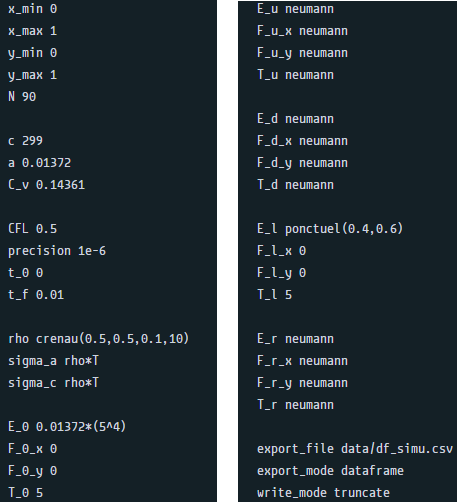
\includegraphics[width=.5\linewidth]{SimuCFG} 
\decoRule
\caption[SimuCFG]{Exemple d'un fichier de configuration. Ici ne sont représentés que les 38 paramètres obligatoires pour faire tourner une simulation et l'exporter. On remarque que le nombre de mailles en horizontale $M$ n'est pas inclu ; il est calculé automatique afin d'obtenir un maillage uniforme. Le résultat produit par ce fichier est présenté aux figures \ref{fig:SimuCIR} et \ref{fig:EvolCIR}.}
\label{fig:SimuCFG}
\end{figure}

\subsection{Sauvegarde des données}

Comme mentionné ci-haut, on dispose de deux options pour sauvegarder les résultats de la simulation :

\begin{itemize}
 \item Sous le forme \textbf{CSV} : ce mode permet une visualisation facile des résultats à l'aide de notebook. Il est très couteux en espace mémoire et nécessite la librairie Pandas pour la lecture sous forme de dataframe. Cette opération est lente et prend une quantité non négligeable de RAM, ce qui peut nuire à l'usage qu'on veut faire des données.
 
 \item Sous le format \textbf{SDS} \footnote{Source - Densité - Signal}: ce format binaire ne sauvegarde que les informations les plus importantes de la simulation. En l'occurrence la source utilisée, la densité du domaine, et les différents signaux sur les bords du domaine. Il est particulièrement intéressant pour générer les données nécessaires à l'apprentissage. Les détails concernant ce format sont donnés en annexe \ref{AppendixA}.
\end{itemize}

%----------------------------------------------------------------------------------------

\section{Résultats}

Quelques résultats obtenus sont présentés ici. Le premier résultat (figures \ref{fig:SimuCIR} et \ref{fig:EvolCIR}) est obtenu avec le fichier de configuration de la figure \ref{fig:SimuCFG}. La source est une onde sinusoïdale placée en $E$ sur une portion de la gauche. La densité a la forme d'un signal en créneau égale à 10 sur le créneau et 0.1 en dehors. Les opacités d'absorption et de dispersion sont proportionnelles à la densité.

\begin{figure}[!h]
\centering
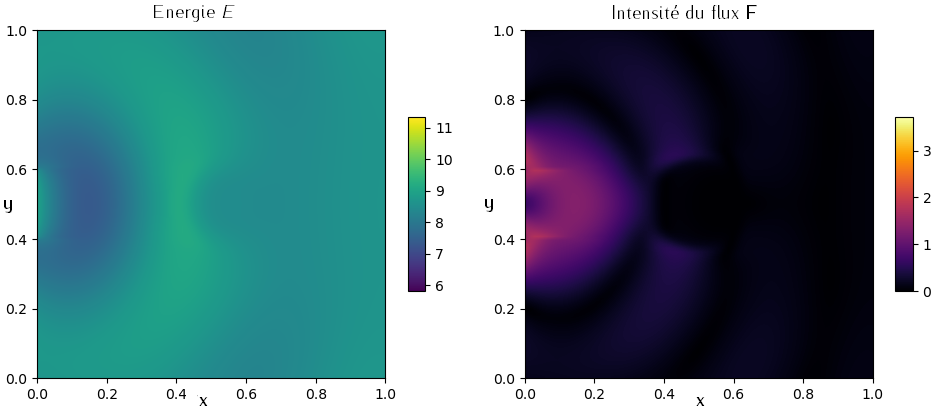
\includegraphics[width=.7\linewidth]{SimuCIR} 
\decoRule
\caption[SimuCIR]{Visualisation de l'énergie et de l'intensité du flux des photons au temps final pour un domaine avec une densité en forme de créneau circulaire (vu du haut). Cette figure correspond au résultat obtenus avec la configuration \ref{fig:SimuCFG}.}
\label{fig:SimuCIR}
\end{figure}

La figure \ref{fig:SimuCIR} permet d'observer une absorption presque totale du signal au niveau du créneau due à la forte valeur des opacités d'absorption et de dispersion. En ce sens, le créneau (saut de densité) très opaque agit comme un obstacle à la propagation du signal. L'évolution de l'énergie sur les bords du domaine (figure \ref{fig:EvolCIR}) traduit aussi bien l'effet qu'a la densité sur la propagation du signal.

\begin{figure}[H]
\centering
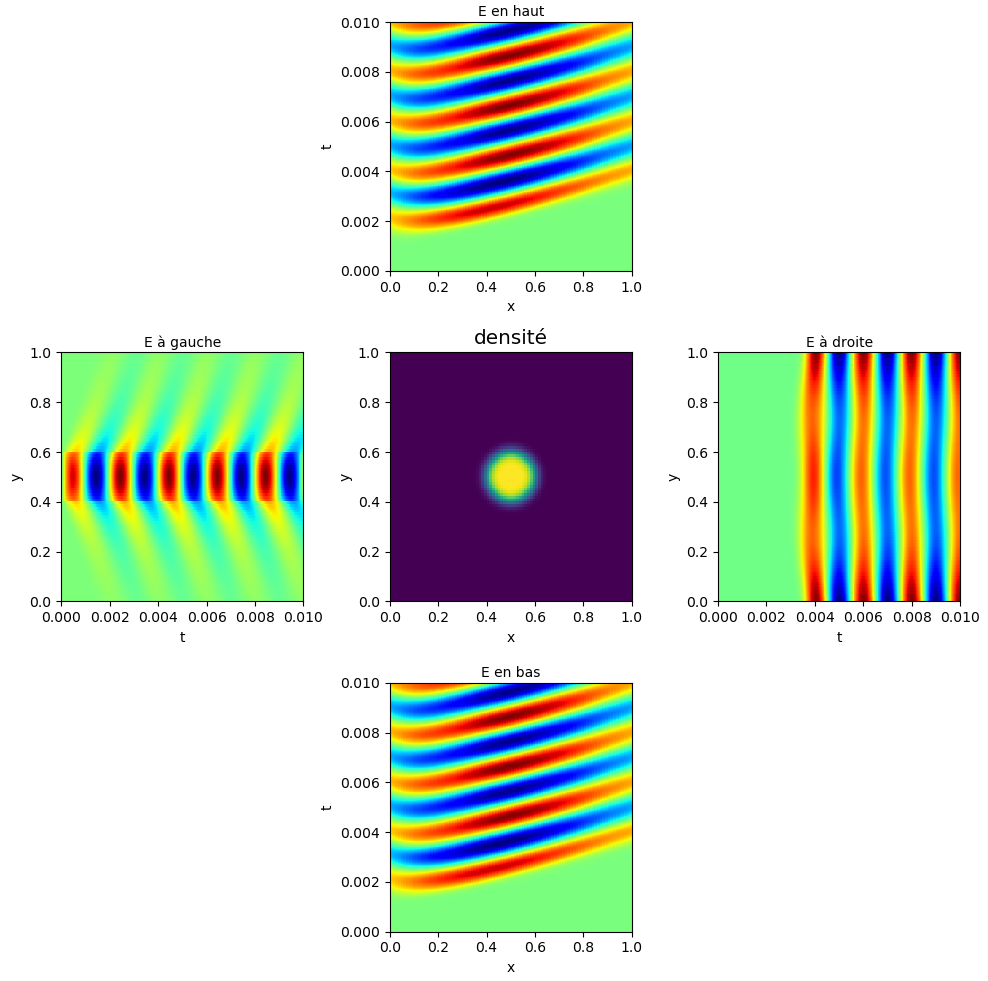
\includegraphics[width=.6\linewidth]{EvolCIR} 
\decoRule
\caption[EvolCIR]{Évolution de l'énergie sur les bords (vue du haut). La cause du problème direct (le saut de densité) est illustrée au milieu de l'image, et son effet sur l'énergie $E$ est présentée aux alentours. Les indices $x$, $y$, et $t$ représentent respectivement l'abscisse, l'ordonnée et le temps. Les autres figures associées à ce cas sont \ref{fig:SimuCFG} et \ref{fig:SimuCIR}.}
\label{fig:EvolCIR}
\end{figure}

Nous testons ensuite notre modèle sur le cas très particulier de l'approximation de diffusion (figures \ref{fig:SimuCFG2}, \ref{fig:SimuREC} et \ref{fig:EvolREC}). Le bord gauche est continûment chauffé ($E_{gauche} = a*((T_{gauche}+1)^4)$). La densité est un signal en forme de créneau rectangulaire (vu du haut) valant 10. En dehors de ce créneau, la densité vaut 0.1. Théoriquement, la limite de diffusion s'observe pour $c/\sigma_c \approx 1$ (voir équation \ref{eqn:Diff}), mais cela pose des problèmes de visualisation en utilisant les coefficients que nous avons choisis. On prend donc $\sigma_a = \sigma_c = 100 \times \rho$ ce qui donne $c / \sigma_c \approx 30$ en dehors de l'obstacle.

On confirme effectivement l'effet de diffusion du signal dans le domaine. Nous pouvons à présent passer à l'apprentissage. Nous nous placerons dans des conditions proches de celles de la configuration \ref{fig:SimuCFG}. L'apprentissage utilisera aussi les données de simulation 1D non présentées ici. Les résultats 1D ont été présentés et analysés dans le rapport de fin de projet de CSMI. 

\begin{figure}[!h]
\centering
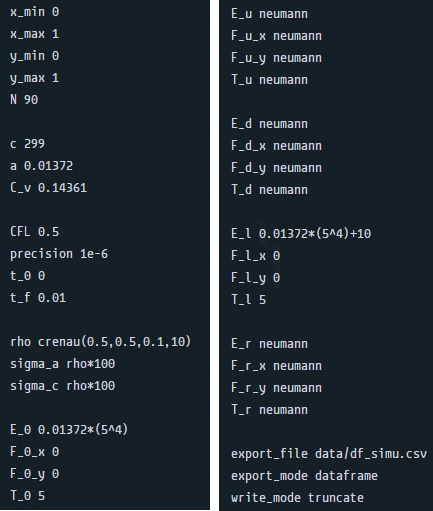
\includegraphics[width=.5\linewidth]{SimuCFG2} 
\decoRule
\caption[SimuCFG2]{Configuration utilisée pour illustrer la limite de diffusion. L'option pour obtenir un obstacle en forme de rectangle n'est pas insérable dans le fichier de configuration, cela se fait directement dans le code de calcul.}
\label{fig:SimuCFG2}
\end{figure}


\begin{figure}[!h]
\centering
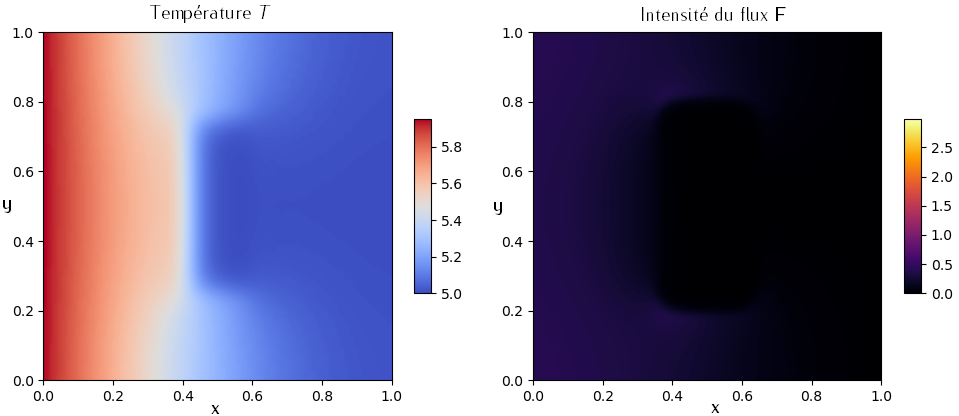
\includegraphics[width=.7\linewidth]{SimuREC} 
\decoRule
\caption[SimuREC]{Visualisation de la température du domaine et de l'intensité du flux des photons au temps final pour la limite de diffusion. La densité à une forme de créneau rectangulaire comme représenté sur l'image du milieu de la figure \ref{fig:EvolREC}.}
\label{fig:SimuREC}
\end{figure}


\begin{figure}[!h]
\centering
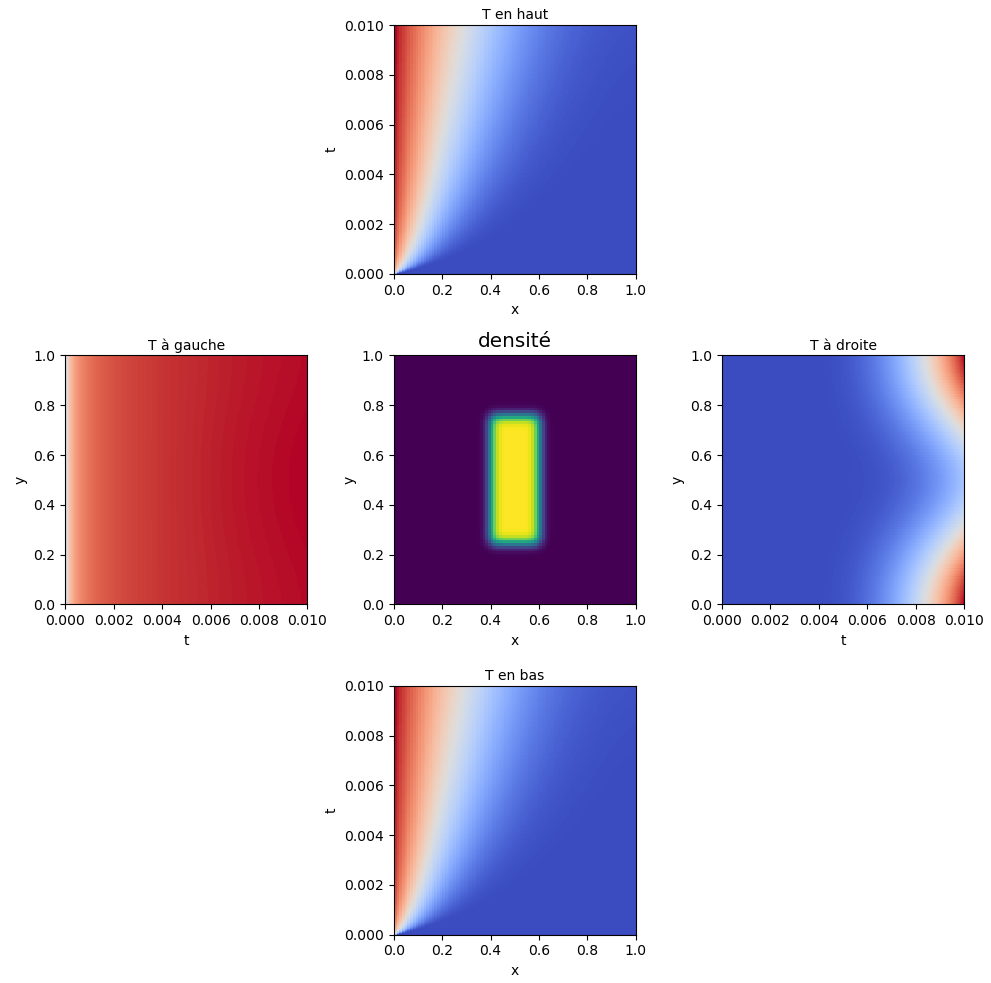
\includegraphics[width=.6\linewidth]{EvolREC} 
\decoRule
\caption[EvolREC]{Évolution de la température sur les bords illustrant l'effet de diffusion. Tout comme à la figure \ref{fig:SimuREC}, l'expression des opacités pour cette simulation est $\sigma_a = \sigma_c = 100 \times \rho$ afin d'obtenir un maximum de diffusion en dehors de l'obstacle mais une absorption totale sur l'obstacle.}
\label{fig:EvolREC}
\end{figure}

%----------------------------------------------------------------------------------------
